\renewcommand*{\arraystretch}{1.1}

\subsection*{BI / read / 23}
\label{sec:bi-read-23}

\noindent\begin{tabularx}{\queryCardWidth}{|>{\queryPropertyCell}c|X|}
	\hline
	query & BI / read / 23 \\ \hline
%
	title & Holiday destinations \\ \hline
%
    pattern & \hfill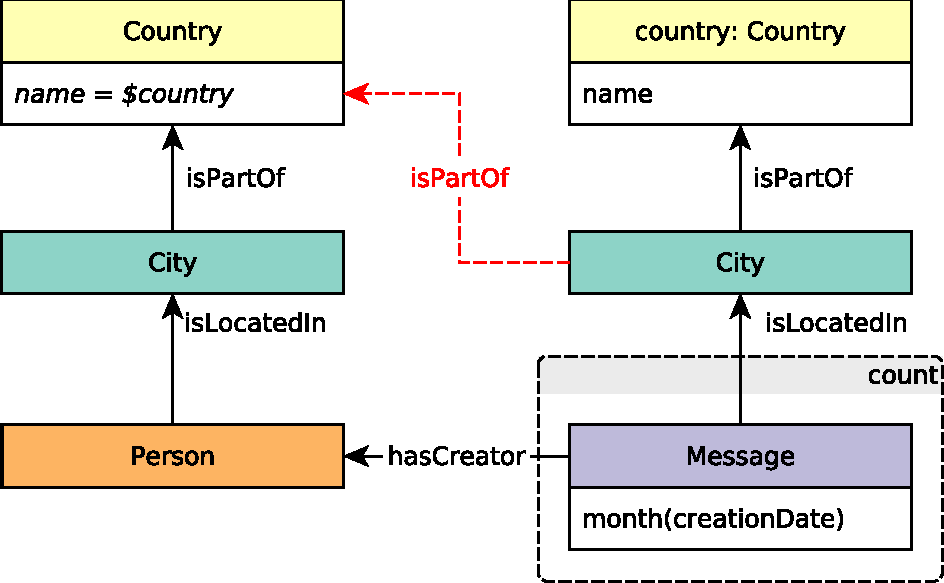
\includegraphics[scale=\patternscale,margin=0cm .2cm]{patterns/bi-read-23}\hfill\vadjust{} \\ \hline
%
	desc. & Count the messages all residents of Country \texttt{country} have
written abroad grouped by month and Country. A Message was written
abroad if the Country the Message was written in is different than the
Country of the Person it was written by.
 \\ \hline
%
	
%
    
        params &
        \innerCardVSpace{\begin{tabularx}{\attributeCardWidth}{|>{\paramNumberCell}c|>{\varNameCell}M|>{\typeCell}m{\typeWidth}|Y|} \hline
        \cellcolor{parameter} \color{white} \footnotesize $\mathsf{1}$ &country& String &  \\ \hline
        \end{tabularx}}\innerCardVSpace \\ \hline
	
%
	
        result &
        \innerCardVSpace{\begin{tabularx}{\attributeCardWidth}{|>{\resultNumberCell}c|>{\varNameCell}M|>{\typeCell}m{\typeWidth}|>{\resultOriginCell}c|Y|} \hline
        $\mathsf{1}$ & messageCount & 32-bit Integer &A&
                The number of messages in each group \\ \hline
        $\mathsf{2}$ & country.name & String &R&
                The name of the destination country \\ \hline
        $\mathsf{3}$ & month & 32-bit Integer &C&
                 \\ \hline
        \end{tabularx}}\innerCardVSpace \\ \hline
	
%
	sort        &
        \innerCardVSpace{\begin{tabular}{|>{\sortNumberCell}c|>{\varNameCell}l|>{\directionCell}c|} \hline
        $\mathsf{1}$ & messageCount & $\desc$ \\ \hline
        $\mathsf{2}$ & country.name & $\asc$ \\ \hline
        $\mathsf{3}$ & month & $\asc$ \\ \hline
        \end{tabular}}\innerCardVSpace \\ \hline
	%
	limit & 100 \\ \hline
	%
	CPs &
	\multicolumn{1}{>{\raggedright}l|}{
	    \chokePoint{1.6}, 
	    \chokePoint{2.3}, 
	    \chokePoint{2.4}, 
	    \chokePoint{3.3}, 
	    \chokePoint{4.3}
	    } \\ \hline
	%
    %
\end{tabularx}
\queryCardVSpace